\documentclass[a4paper]{article}

\usepackage{INTERSPEECH2018}
\usepackage{cite}

\title{Paper Template for INTERSPEECH 2018}
\name{Author Name$^1$, Co-author Name$^2$}
%The maximum number of authors in the author list is twenty. If the number of contributing authors is more than twenty, they should be listed in a footnote or in acknowledgement section, as appropriate.
\address{
  $^1$Author Affiliation\\
  $^2$Co-author Affiliation}
\email{author@university.edu, coauthor@company.com}

\begin{document}

\maketitle
% 
\begin{abstract}
  This report describes the paper \cite{dredze2010nlp} which was presented by me and two other papers: \cite{Davis80-COP} and \cite{Davis80-COP}. For your paper to be published in the conference proceedings, you must use this document as both an instruction set and as a template into which you can type your own text. If your paper does not conform to the required format, you will be asked to fix it.

  Please do not reuse your past papers as a template. To prepare your paper for submission, please always download a fresh copy of this template from the conference website and please read the format instructions in this template before you use it for your paper.

  Conversion to PDF may cause problems in the resulting PDF or expose problems in your source document. Before submitting your final paper in PDF, check that the format in your paper PDF conforms to this template. Specifically, check the appearance of the title and author block, the appearance of section headings, document margins, column width, column spacing, and other features such as figure numbers, table numbers and equation number. In summary, you must proofread your final paper in PDF before submission.
  
  The maximum number of pages is 5. The 5\textsuperscript{th} page may be used exclusively for references. The references should begin on an earlier page immediately after the Acknowledgements section, and continue onto the 5\textsuperscript{th} page. If no space is available on an earlier page, then the references may begin on the 5\textsuperscript{th} page.

  Index terms should be included as shown below.
\end{abstract}
\noindent\textbf{Index Terms}: speech recognition, human-computer interaction, computational paralinguistics

\section{Introduction}

This template can be found on the conference website. Templates are provided for Microsoft Word\textregistered, and \LaTeX. However, we highly recommend using \LaTeX when preparing your submission. Information for full paper submission is available on the conference website.

\section{Page layout and style}

Authors should observe the following rules for page layout. A highly recommended way to meet these requirements is to use a given template (Microsoft Word® or LaTeX) and check details against the corresponding example PDF file. Given templates, Microsoft Word\textregistered\ or \LaTeX, can be adapted/imported easily in other software such as LibreOffice, Apple Pages, Lua\LaTeX, and Xe\LaTeX, but please be careful to match the layout of the provided PDF example.

\subsection{Basic layout features}

\begin{itemize}
\item Proceedings will be printed in DIN A4 format. Authors must submit their papers in DIN A4 format.
\item Two columns are used except for the title section and for large figures that may need a full page width.
\item Left and right margin are 20 mm each. 
\item Column width is 80 mm. 
\item Spacing between columns is 10 mm.
\item Top margin is 25 mm (except for the first page which is 30 mm to the title top).
\item Bottom margin is 35 mm.
\item Text height (without headers and footers) is maximum 235 mm.
\item Headers and footers must be left empty.
\item Check indentations and spacings by comparing to this example file (in PDF).
\end{itemize}

\subsubsection{Headings}

Section headings are centered in boldface with the first word capitalized and the rest of the heading in lower case. Sub- headings appear like major headings, except they start at the left margin in the column. Sub-sub-headings appear like sub-headings, except they are in italics and not boldface. See the examples in this file. No more than 3 levels of headings should be used.

\subsection{Text font}

Times or Times Roman font is used for the main text. Font size in the main text must be 9 points, and in the References section 8 points. Other font types may be used if needed for special purposes. It is VERY IMPORTANT that while making the final PDF file, you embed all used fonts! To embed the fonts, you may use the following instructions:
\begin{enumerate}
\item For Windows users, the bullzip printer can convert any PDF to have embedded and subsetted fonts.
\item For Linux/Mac users, you may use \\
   pdftops file.pdf\\
   pstopdf -dPDFSETTINGS=/prepress file.pdf
\end{enumerate}

\LaTeX users: users should use Adobe Type 1 fonts such as Times or Times Roman. These are used automatically by the INTERSPEECH2018.sty style file. Authors must not use Type 3 (bitmap) fonts.

\subsection{Figures}

All figures must be centered on the column (or page, if the figure spans both columns). Figure captions should follow each figure and have the format given in
% Figure~\ref{fig:speech_production}.

Figures should be preferably line drawings. If they contain gray levels or colors, they should be checked to print well on a high-quality non-color laser printer.

Graphics (i.\,e., illustrations, figures) must not use stipple fill patterns because they will not reproduce properly in Adobe PDF. Please use only SOLID FILL COLORS.

Figures which span 2 columns (i.\,e., occupy full page width) must be placed at the top or bottom of the page.

\subsection{Tables}

An example of a table is shown in Table ~\ref{tab:example}. The caption text must be above the table.

\begin{table}[th]
  \caption{This is an example of a table}
  \label{tab:example}
  \centering
  \begin{tabular}{ r@{}l  r }
    \toprule
    \multicolumn{2}{c}{\textbf{Ratio}} & 
                                         \multicolumn{1}{c}{\textbf{Decibels}} \\
    \midrule
    $1$                       & $/10$ & $-20$~~~             \\
    $1$                       & $/1$  & $0$~~~               \\
    $2$                       & $/1$  & $\approx 6$~~~       \\
    $3.16$                    & $/1$  & $10$~~~              \\
    $10$                      & $/1$  & $20$~~~              \\
    $100$                     & $/1$  & $40$~~~              \\
    $1000$                    & $/1$  & $60$~~~              \\
    \bottomrule
  \end{tabular}
  
\end{table}

\subsection{Equations}

Equations should be placed on separate lines and numbered. Examples of equations are given below. Particularly,
% 
\begin{equation}
  x(t) = s(f_\omega(t))
  \label{eq1}
\end{equation}
% 
where \(f_\omega(t)\) is a special warping function
% 
\begin{equation}
  f_\omega(t) = \frac{1}{2 \pi j} \oint_C 
  \frac{\nu^{-1k} \mathrm{d} \nu}
  {(1-\beta\nu^{-1})(\nu^{-1}-\beta)}
  \label{eq2}
\end{equation}
% 
A residue theorem states that
% 
\begin{equation}
  \oint_C F(z)\,\mathrm{d}z = 2 \pi j \sum_k \mathrm{Res}[F(z),p_k]
  \label{eq3}
\end{equation}
% 
Applying (\ref{eq3}) to (\ref{eq1}), it is straightforward to see that
% 
\begin{equation}
  1 + 1 = \pi
  \label{eq4}
\end{equation}

Finally we have proven the secret theorem of all speech sciences. No more math is needed to show how useful the result is!

% \begin{figure}[t]
%   \centering
%   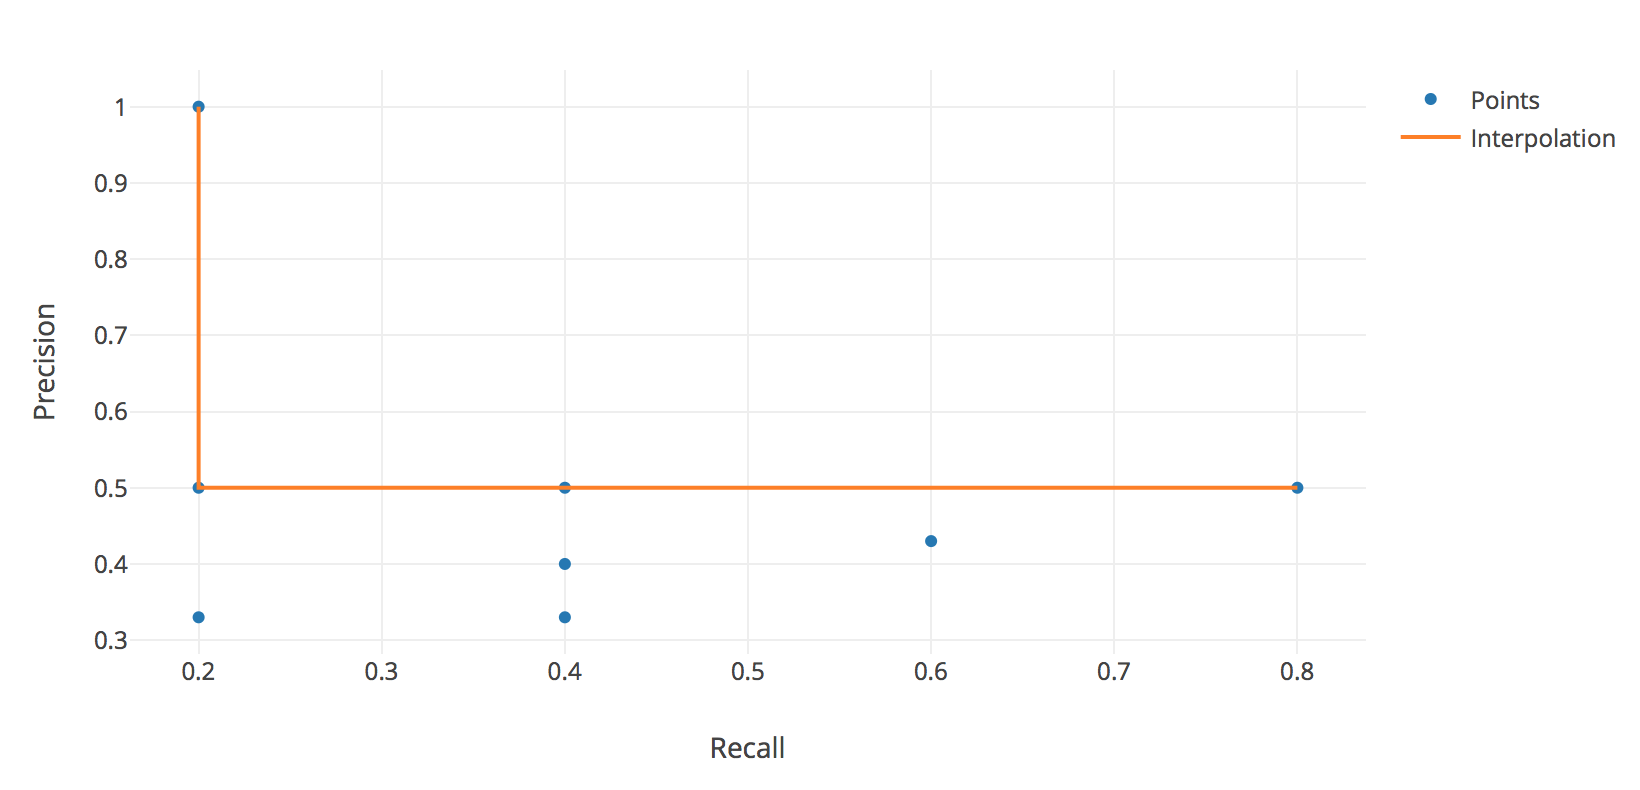
\includegraphics[width=\linewidth]{figure.pdf}
%   \caption{Schematic diagram of speech production.}
%   \label{fig:speech_production}
% \end{figure}

\subsection{Information for Word users only}

For ease of formatting, please use the styles listed in Table 2. The styles are defined in this template file and are shown in the order in which they would be used when writing a paper. When the heading styles in Table 2 are used, section numbers are no longer required to be typed in because they will be automatically numbered by Word. Similarly, reference items will be automatically numbered by Word when the ``Reference'' style is used.

\begin{table}[t]
  \caption{Main predefined styles in Word}
  \label{tab:word_styles}
  \centering
  \begin{tabular}{ll}
    \toprule
    \textbf{Style Name}      & \textbf{Entities in a Paper}                \\
    \midrule
    Title                    & Title                                       \\
    Author                   & Author name                                 \\
    Affiliation              & Author affiliation                          \\
    Email                    & Email address                               \\
    AbstractHeading          & Abstract section heading                    \\
    Body Text                & First paragraph in abstract                 \\
    Body Text Next           & Following paragraphs in abstract            \\
    Index                    & Index terms                                 \\
    1. Heading 1             & 1\textsuperscript{st} level section heading \\
    1.1 Heading 2            & 2\textsuperscript{nd} level section heading \\
    1.1.1 Heading 3          & 3\textsuperscript{rd} level section heading \\
    Body Text                & First paragraph in section                  \\
    Body Text Next           & Following paragraphs in section             \\
    Figure Caption           & Figure caption                              \\
    Table Caption            & Table caption                               \\
    Equation                 & Equations                                   \\
    \textbullet\ List Bullet & Bulleted lists                              \\\relax
    [1] Reference            & References                                  \\
    \bottomrule
  \end{tabular}
\end{table}

If your Word document contains equations, you must not save your Word document from ``.docx'' to ``.doc'' because when doing so, Word will convert all equations to images of unacceptably low resolution.

\subsection{Hyperlinks}

For technical reasons, the proceedings editor will strip all active links from the papers during processing. Hyperlinks can be included in your paper, if written in full, e.\,g.\ ``http://www.foo.com/index.html''. The link text must be all black. 
Please make sure that they present no problems in printing to paper.

\subsection{Multimedia files}

The INTERSPEECH organizing committee offers the possibility to submit multimedia files.

\subsection{Page numbering}

Final page numbers will be added later to the document electronically. \emph{Don't make any footers or headers!}


\subsection{References}

The reference format is the standard IEEE one. References should be numbered in order of appearance, for example \cite{Davis80-COP}, \cite{Rabiner89-ATO}, \cite[pp.\ 417--422]{Hastie09-TEO}, and \cite{YourName17-XXX}.

\subsection{Abstract}

The total length of the abstract is limited to 200 words. The abstract included in your paper and the one you enter during web-based submission must be identical. Avoid non-ASCII characters or symbols as they may not display correctly in the abstract book.

\subsection{Author affiliation}

Please list country names as part of the affiliation for each country.

\subsection{Number of authors in the author list}

The maximum number of authors in the author list is twenty. If the number of contributing authors is more than twenty, they should be listed in a footnote or in acknowledgement section, as appropriate.

\subsection{Submitted files}

Authors are requested to submit PDF files of their manu­scripts. 

\section{Discussion}

This is the discussion. This is the discussion. This is the discussion. Is there any discussion?

\section{Conclusions}

Authors must proofread their PDF file prior to submission to ensure it is correct. Authors should not rely on proofreading the Word file. Please proofread the PDF file before it is submitted.

\section{Acknowledgements}

The ISCA Board would like to thank the organizing committees of the past INTERSPEECH conferences for their help and for kindly providing the template files. \\
Note to authors: Authors should not use logos in acknowledgement section; rather authors should acknowledge corporations by naming them only.


\bibliographystyle{IEEEtran}

\bibliography{mybib}

% \begin{thebibliography}{9}
% \bibitem[1]{Davis80-COP}
%   S.\ B.\ Davis and P.\ Mermelstein,
%   ``Comparison of parametric representation for monosyllabic word recognition in continuously spoken sentences,''
%   \textit{IEEE Transactions on Acoustics, Speech and Signal Processing}, vol.~28, no.~4, pp.~357--366, 1980.
% \bibitem[2]{Rabiner89-ATO}
%   L.\ R.\ Rabiner,
%   ``A tutorial on hidden Markov models and selected applications in speech recognition,''
%   \textit{Proceedings of the IEEE}, vol.~77, no.~2, pp.~257-286, 1989.
% \bibitem[3]{Hastie09-TEO}
%   T.\ Hastie, R.\ Tibshirani, and J.\ Friedman,
%   \textit{The Elements of Statistical Learning -- Data Mining, Inference, and Prediction}.
%   New York: Springer, 2009.
% \bibitem[4]{YourName17-XXX}
%   F.\ Lastname1, F.\ Lastname2, and F.\ Lastname3,
%   ``Title of your INTERSPEECH 2018 publication,''
%   in \textit{Interspeech 2018 -- 19\textsuperscript{th} Annual Conference of the International Speech Communication Association, September 2-6, Hyderabad, India Proceedings, Proceedings}, 2018, pp.~100--104.
% \end{thebibliography}

\end{document}
